\documentclass{article}
\usepackage[utf8]{inputenc}
\usepackage[catalan]{babel}
\usepackage{amssymb}        % símbols de l'AMS
\usepackage{amsmath}        % macros de l'AMS
\usepackage[pdftex]{graphicx}  % poder incloure gráfics
\usepackage[pdftex]{color}     % poder fer servir color al text
\usepackage{multicol}
\usepackage{amsthm}
\usepackage{listings}
\usepackage{hyperref}
\usepackage{geometry}
\usepackage{tikz}
\usepackage{pgfplots}
\usepackage{subcaption}
\usepackage[catalan]{babel}
\usepackage{mathtools}
\usepackage{geometry}
\usepackage{amsmath}
\usepackage{amssymb}
\usepackage{fancyhdr}
\usepackage{multirow}
%\usepackage[table,xcdraw]{xcolor}
\usepackage{float}
\usepackage{verbatim}
\usepackage{pgfplots}
\pgfplotsset{compat=newest}
\usepgfplotslibrary{fillbetween}
\usetikzlibrary{patterns}
\usepackage{vmargin} 				%margenes



\title{Pràctica 1: Regressió}
\author{Guillermo Vivancos Alonso 1606206\\
	Javier Esmoris Cerezuela 1498396\\
	Oriol Marión Escudé 1566740}
\begin{document}
\date{}
\setpapersize{A4}
\setmargins{2.5cm}       % margen izquierdo
{1.5cm}                        % margen superior
{16.5cm}                      % anchura del texto
{23.35cm}                    % altura del texto
{10pt}                           % altura de los encabezados
{1cm}                           % espacio entre el texto y los encabezados
{0pt}                             % altura del pie de página
{2cm}                           % espacio entre el texto y el pie de página

\pagestyle{fancy}
\fancyhf{}
\lhead{\textbf{Aprenentatge Computacional 102787} \newline Pràctica 1: Regressió\\}
\rhead{\hfill \textbf{
		Guillermo Vivancos Alonso 1606206\\
		Javier Esmoris Cerezuela 1498396\\
		Oriol Marión Escudé 1566740}}
\rfoot{\thepage}
\maketitle
\noindent
\section*{Introducció}
En aquesta pràctica analitzarem una base de dades sobre els partits que ha jugat Michael Jordan. Veurem quines distribucions tenen els atributs, la relació entre ells i intentarem predir els punts que farà en un partit.

\section*{Apartat C}
Els atributs que tenim a la base de dades són els següents:
\begin{enumerate}
	\addtocounter{enumi}{-1}
	\item Game [integer]: ID del partit.
	\item Date [string]: data del partit en el format "yyyy/mm/dd".
	\item Age [string]: edat del jugador mesurada en anys i dies.
	\item Team [string]: equip al que pertany el jugador. 
	\item Opp [string]: equip adversari en el partit.
	\item Result [string]: diferència de punts del equip respecte l'adversari, acompanyat d'una lletra Win/Lose.
	\item mp [string]: minuts jugats amb el format "mm:ss"
	\item fg [integer]: tirs anotats.
	\item fga [integer]: tirs intentats.
	\item fgp [float]: freqüència relativa de tirs anotats.
	\item three [integer]: triples anotats.
	\item threeatt [integer]: triples intentats.
	\item threep [float]: freqüència relativa de triples anotats.
	\item ft [integer]: tirs lliures anotats.
	\item fta [integer]: tirs lliures intentats.
	\item ftp [float]: freqüència relativa de tirs lliures anotats.
	\item orb [integer]: rebots ofensius.
	\item drb [integer]: rebots defensius.
	\item trb [integer]: rebots totals.
	\item ast [integer]: assistències.
	\item stl [integer]: pilotes robades
	\item blk [integer]: llançaments de dos punts bloquejats.
	\item tov [integer]: pilotes perdudes.
	\item pts [integer]: punts aconseguits pel jugador.
	\item game\_score [float]: mitjana de punts de l'equip per jugador.
	\item minus\_plus [NaN]: diferència en el marcador respecte la entrada i la sortida del jugador.
\end{enumerate}
No cal netejar massa la base de dades, només hi ha tres atributs on trobem \textit{NaNs}. Els dos primers són \textit{threep} i \textit{ftp}, freqüències relatives de triples i tirs lliures respectivament, que no estan definits si no hi ha hagut cap intent (divisió per zero). L'últim atribut amb \textit{NaNs} és \textit{minus\_plus}, que té tots els valors sense definir i, per tant, descartarem aquest atribut.
\\
\\
%Quins atributs tenen una distribució Guassiana?\\
Per veure quins atributs segueixen una distribució Gaussiana hem fet histogrames i tests d'hipòtesi.
A simple vista, els atributs que més s'assemblen a una distribució normal són els tres atributs pels tirs, els punts i el game\_score. Hem fet els testos de normalitat a totes les variables però a les taules només veurem aquests cinc atributs.
\\
\begin{figure}[!h]
	\centering
	\begin{subfigure}[b]{0.25\textwidth}
		\centering
		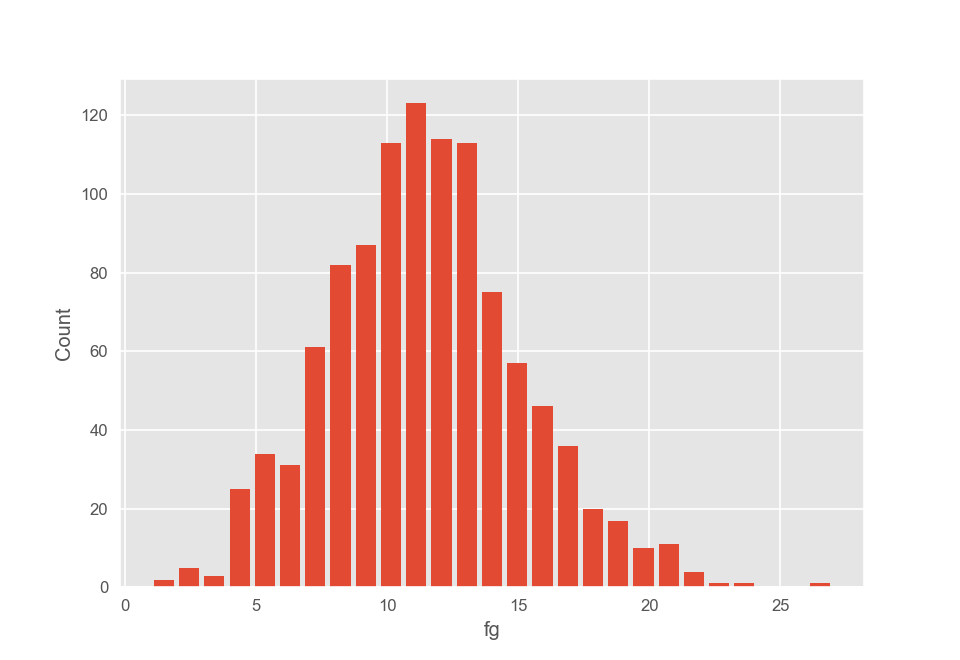
\includegraphics[width=\textwidth]{hist7}
		\caption*{Anotats}
		\label{fig:hist7}
	\end{subfigure}
	\hfill
	\begin{subfigure}[b]{0.25\textwidth}
		\centering
		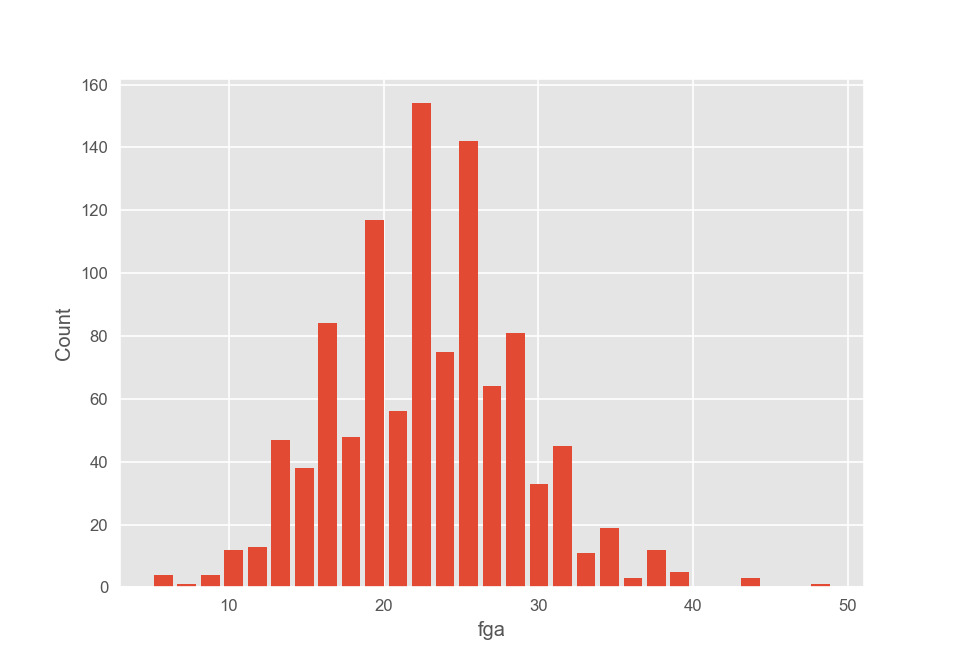
\includegraphics[width=\textwidth]{hist8}
		\caption*{Intentats}
		\label{fig:hist8}
	\end{subfigure}
	\hfill
	\begin{subfigure}[b]{0.25\textwidth}
		\centering
		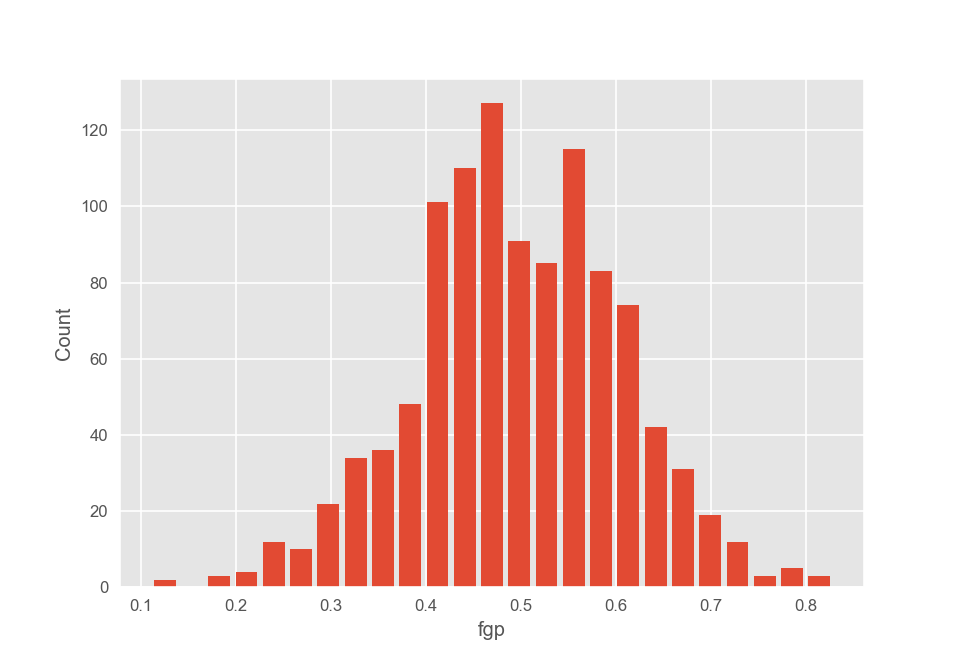
\includegraphics[width=\textwidth]{hist9}
		\caption*{Freqüència relativa}
		\label{fig:hist9}
	\end{subfigure}
	\caption{Tirs}
	\label{fig:tirs}
\end{figure}
\begin{figure}[!h]
	\centering
	\begin{subfigure}[b]{0.25\textwidth}
		\centering
		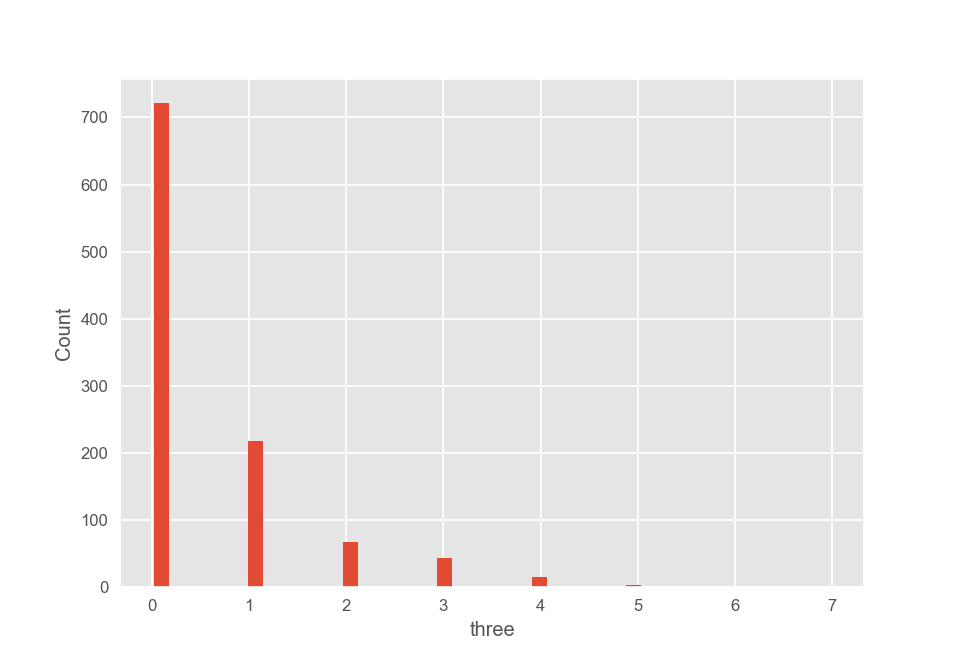
\includegraphics[width=\textwidth]{hist10}
		\caption*{Anotats}
		\label{fig:hist10}
	\end{subfigure}
	\hfill
	\begin{subfigure}[b]{0.25\textwidth}
		\centering
		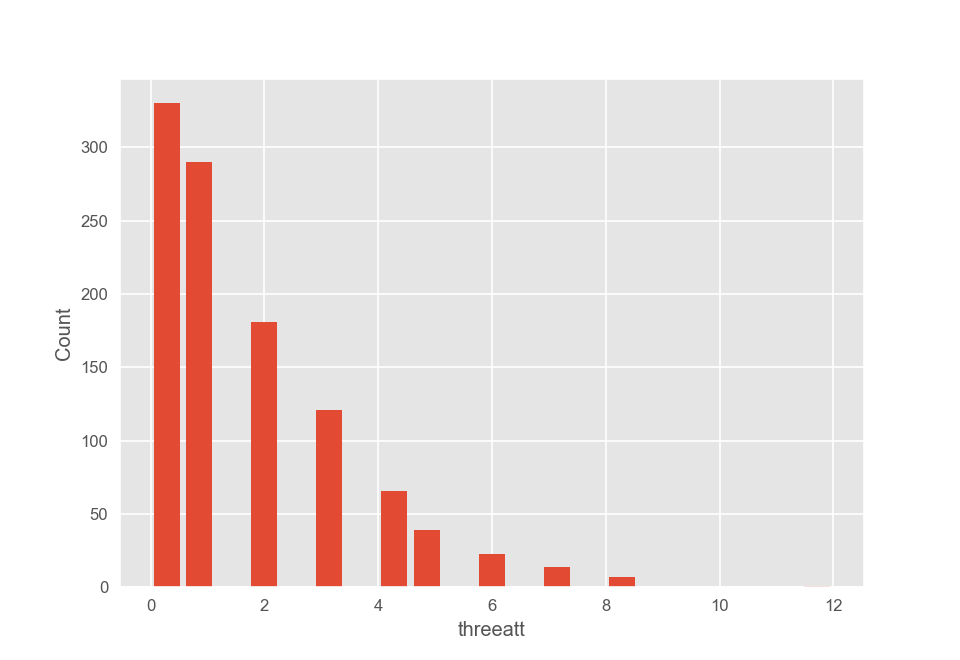
\includegraphics[width=\textwidth]{hist11}
		\caption*{Intentats}
		\label{fig:hist11}
	\end{subfigure}
	\hfill
	\begin{subfigure}[b]{0.25\textwidth}
		\centering
		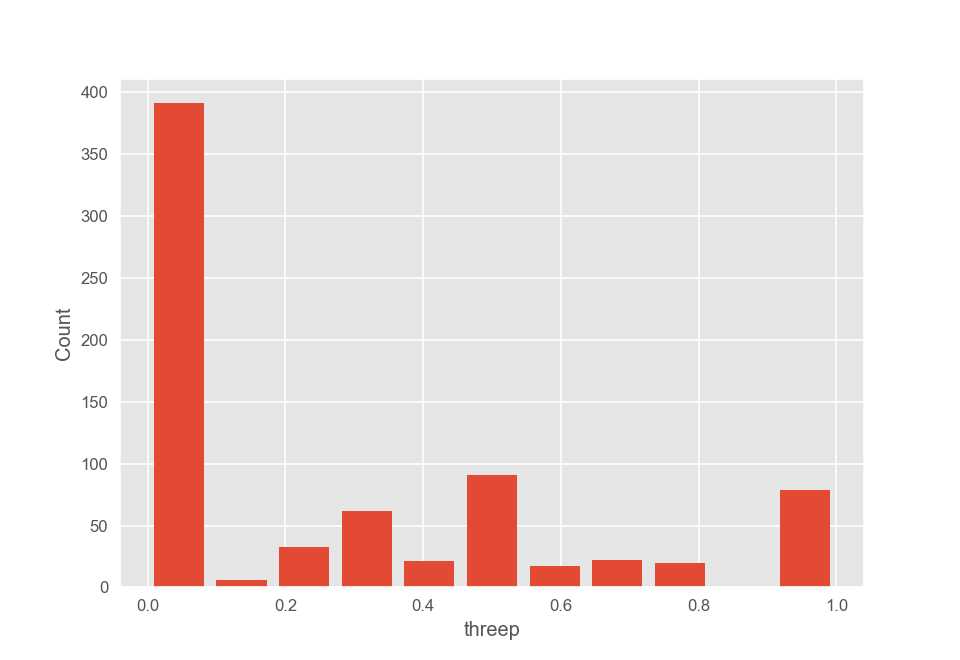
\includegraphics[width=\textwidth]{hist12}
		\caption*{Freqüència relativa}
		\label{fig:hist12}
	\end{subfigure}
	\caption{Triples}
	\label{fig:triples}
\end{figure}
\begin{figure}[!h]
	\centering
	\begin{subfigure}[b]{0.25\textwidth}
		\centering
		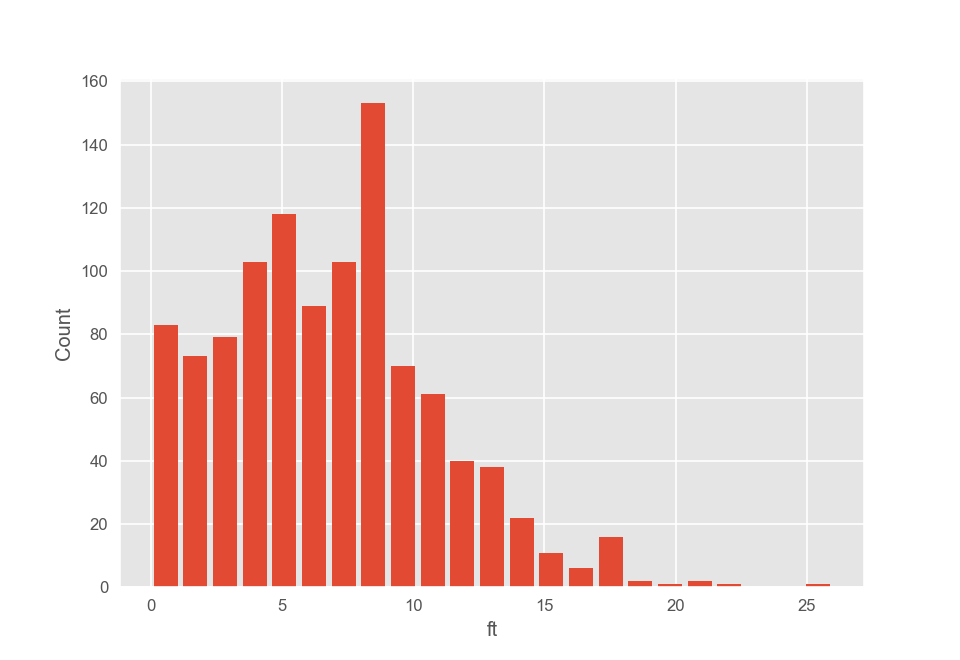
\includegraphics[width=\textwidth]{hist13}
		\caption*{Anotats}
		\label{fig:hist13}
	\end{subfigure}
	\hfill
	\begin{subfigure}[b]{0.25\textwidth}
		\centering
		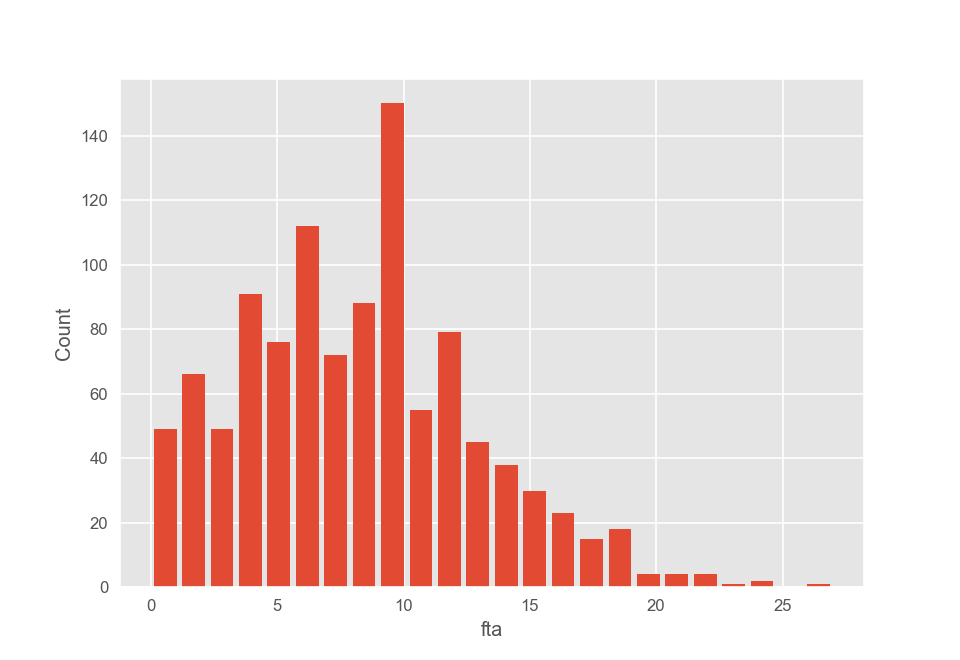
\includegraphics[width=\textwidth]{hist14}
		\caption*{Intentats}
		\label{fig:hist14}
	\end{subfigure}
	\hfill
	\begin{subfigure}[b]{0.25\textwidth}
		\centering
		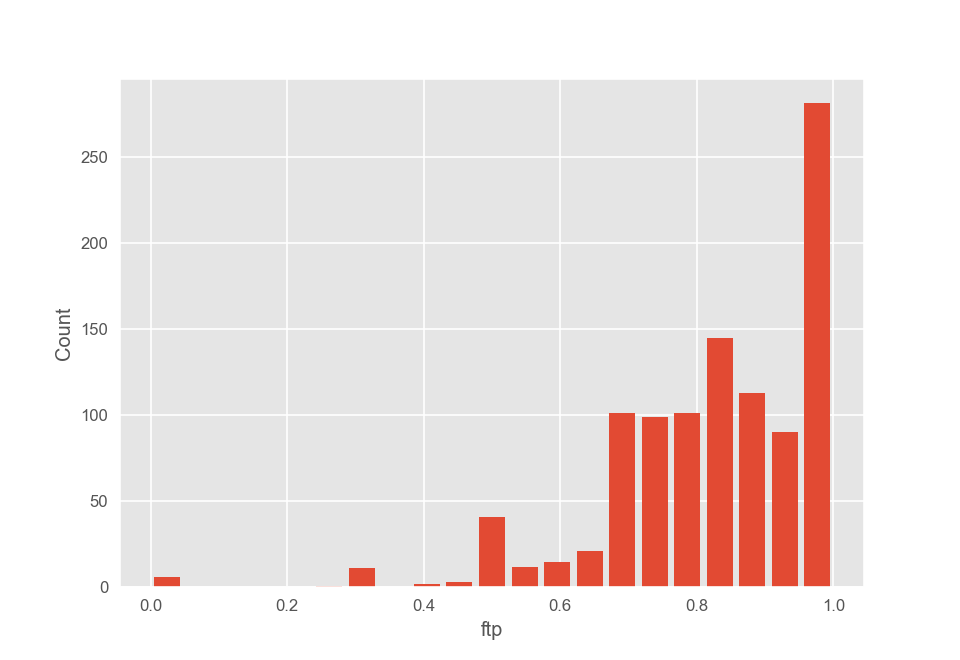
\includegraphics[width=\textwidth]{hist15}
		\caption*{Freqüència relativa}
		\label{fig:hist15}
	\end{subfigure}
	\caption{Tirs lliures}
	\label{fig:tirs}
\end{figure}
\begin{figure}[!h]
	\centering
	\begin{subfigure}[b]{0.25\textwidth}
		\centering
		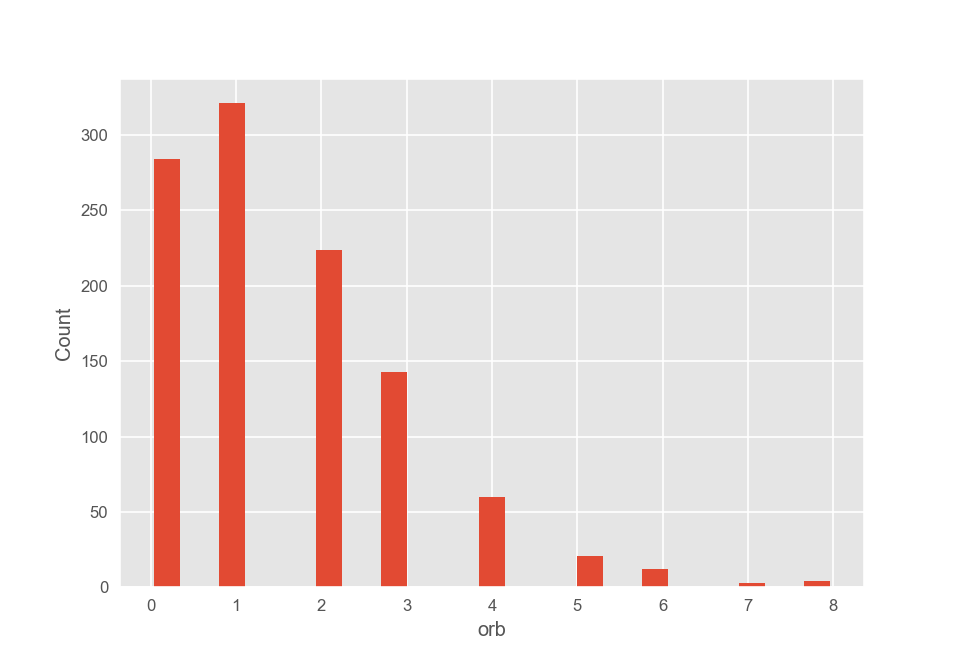
\includegraphics[width=\textwidth]{hist16}
		\caption*{Ofensius}
		\label{fig:hist16}
	\end{subfigure}
	\hfill
	\begin{subfigure}[b]{0.25\textwidth}
		\centering
		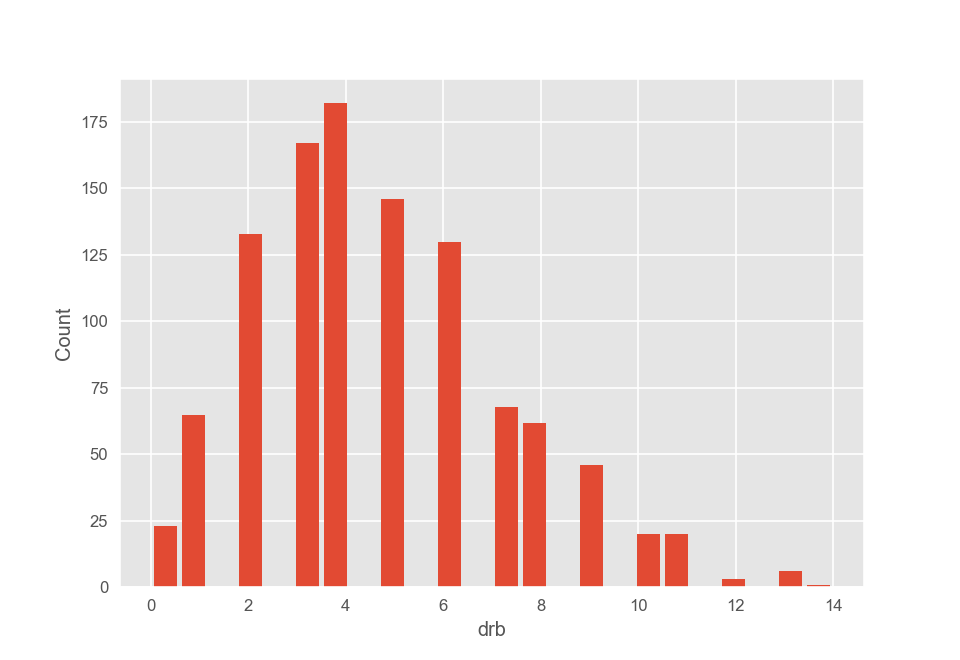
\includegraphics[width=\textwidth]{hist17}
		\caption*{Defensius}
		\label{fig:hist17}
	\end{subfigure}
	\hfill
	\begin{subfigure}[b]{0.25\textwidth}
		\centering
		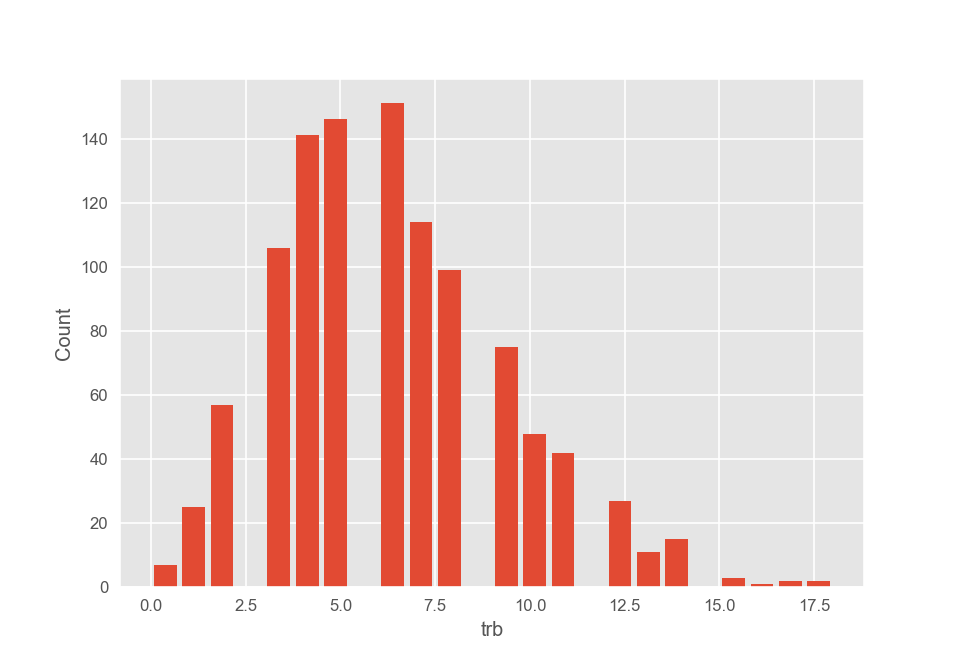
\includegraphics[width=\textwidth]{hist18}
		\caption*{Totals}
		\label{fig:hist18}
	\end{subfigure}
	\caption{Rebots}
	\label{fig:tirs}
\end{figure}
\begin{figure}[!h]
	\centering
	\begin{subfigure}[b]{0.25\textwidth}
		\centering
		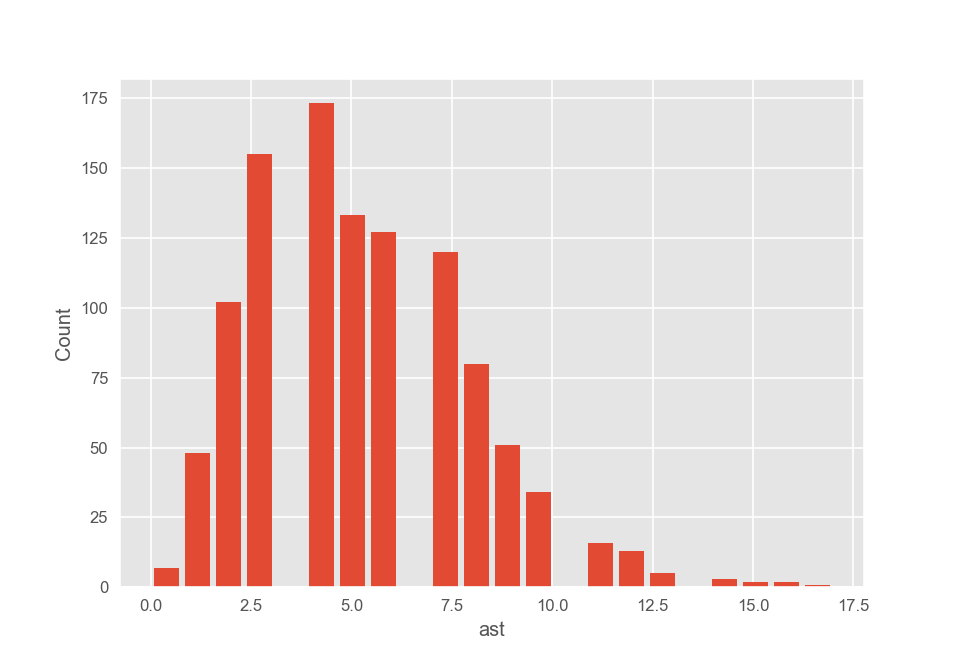
\includegraphics[width=\textwidth]{hist19}
		\caption*{Asistències}
		\label{fig:hist19}
	\end{subfigure}
	\hfill
	\begin{subfigure}[b]{0.25\textwidth}
		\centering
		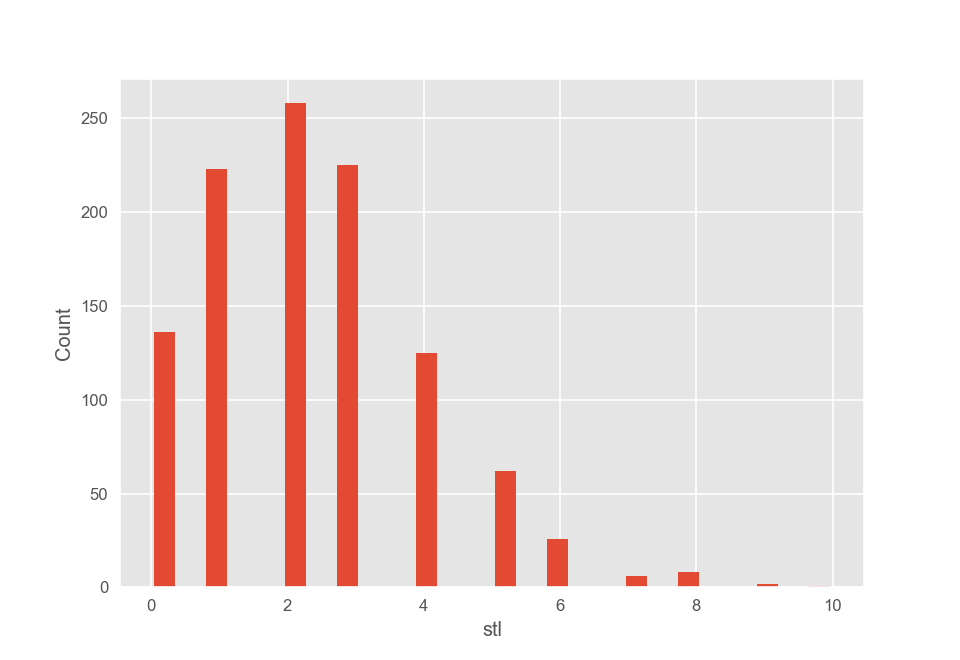
\includegraphics[width=\textwidth]{hist20}
		\caption*{Boles robades}
		\label{fig:hist20}
	\end{subfigure}
	\hfill
	\begin{subfigure}[b]{0.25\textwidth}
		\centering
		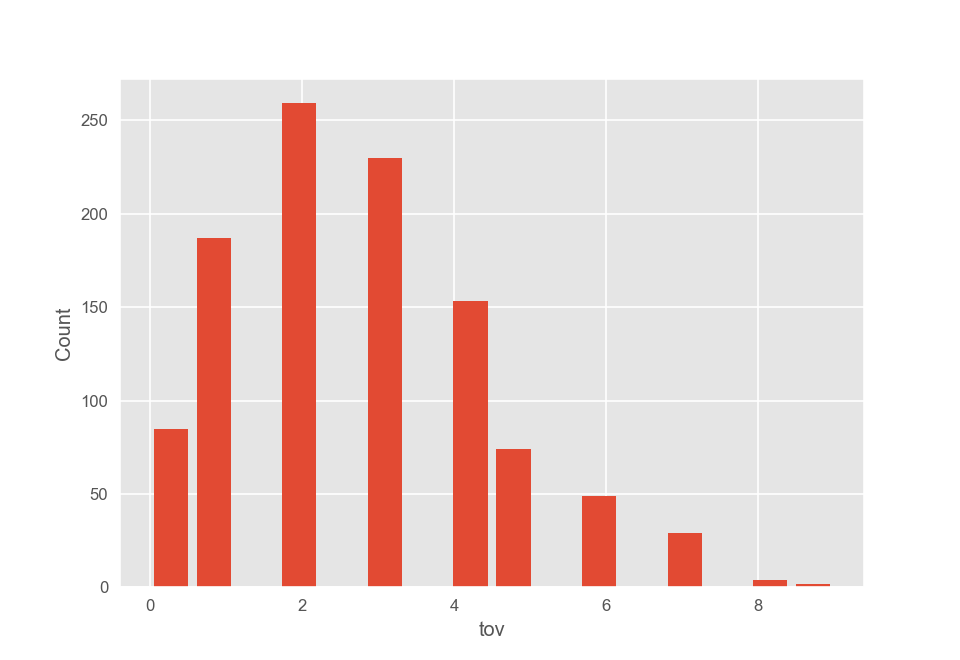
\includegraphics[width=\textwidth]{hist22}
		\caption*{Boles perdudes}
		\label{fig:hist22}
	\end{subfigure}
	\caption{Asistències, boles robades i perdudes}
	\label{fig:hist20}
\end{figure}
\begin{figure}[!h]
	\centering
	\begin{subfigure}[b]{0.25\textwidth}
		\centering
		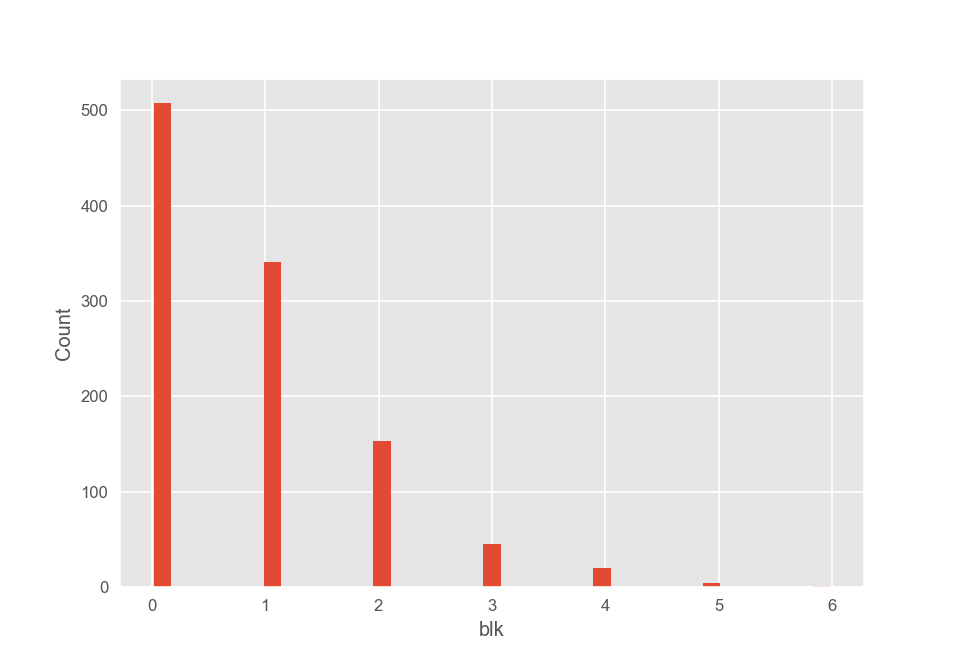
\includegraphics[width=\textwidth]{hist21}
		\caption*{Bloquejos}
		\label{fig:hist21}
	\end{subfigure}
	\hfill
	\begin{subfigure}[b]{0.25\textwidth}
		\centering
		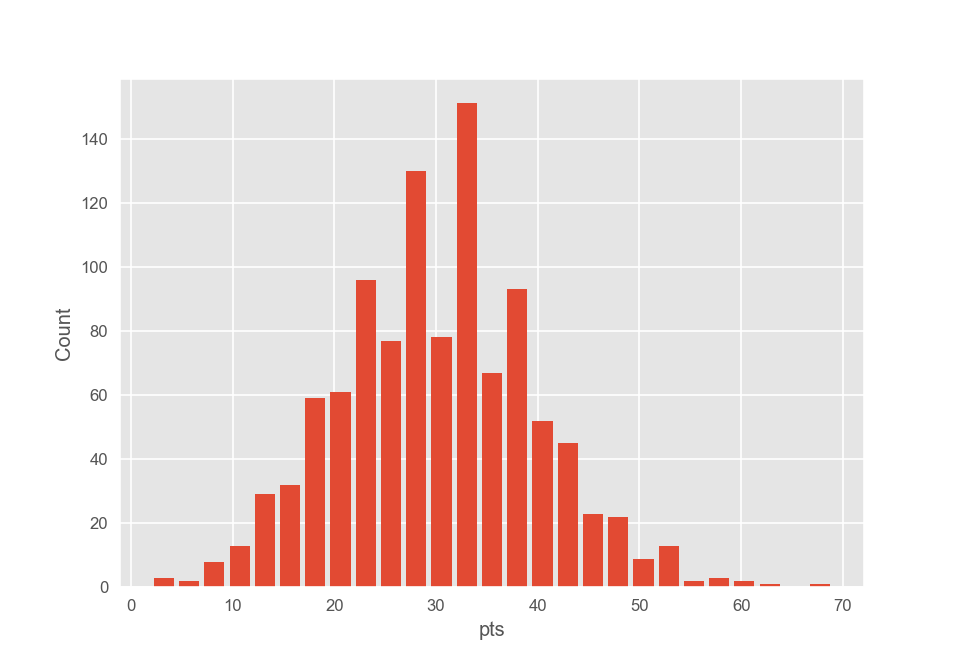
\includegraphics[width=\textwidth]{hist23}
		\caption*{Punts}
		\label{fig:hist23}
	\end{subfigure}
	\hfill
	\begin{subfigure}[b]{0.25\textwidth}
		\centering
		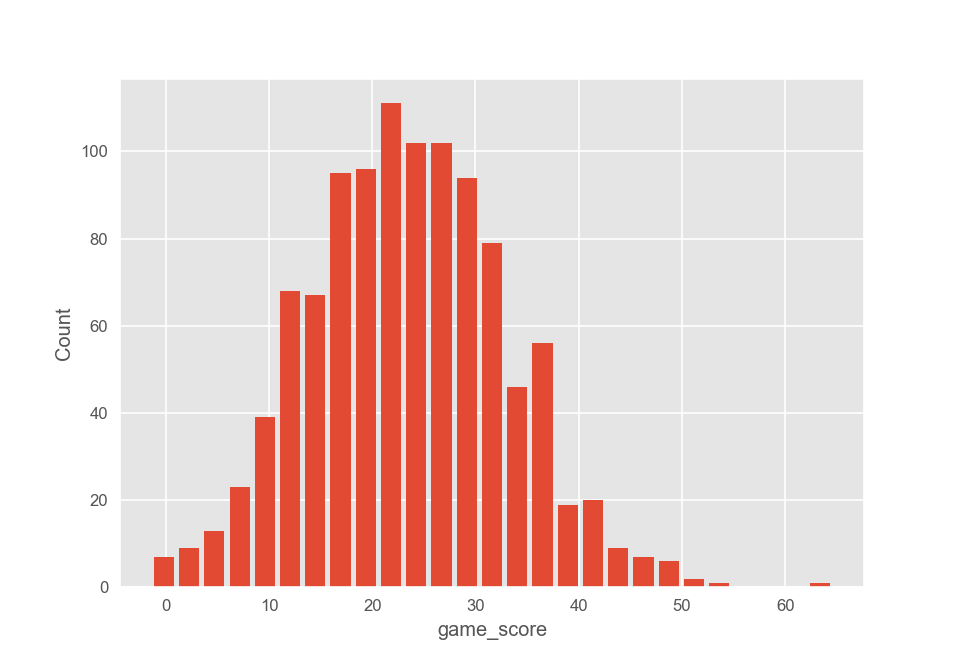
\includegraphics[width=\textwidth]{hist24}
		\caption*{Game\_score}
		\label{fig:hist24}
	\end{subfigure}
	\caption{Bloquejos, punts i game\_score}
	\label{fig:hist20}
\end{figure}
%Quin és l'atribut objectiu? Per què?\\
\\
%7,8,9,23,24
\begin{table}[h!]
	\begin{center}
		\begin{tabular}{| c | c | c | c | c |}\hline
			Atribut & Estadístic Shapiro & $p$ Phapiro & Estadístic Agostino $K^2$ & $p$ Agostino $K^2$ \\ \hline
			fg & 0.989 & 0.000 & 14.586 & 0.001 \\ \hline
			fga & 0.993 & 0.000 & 12.643 & 0.002 \\ \hline
			fgp & 0.998 & 0.119 & 2.2689 & 0.261 \\ \hline
			pts & 0.996 & 0.014 & 7.417 & 0.024 \\ \hline
			game\_score & 0.997 & 0.030 & 7.417 & 0.025 \\ \hline
		\end{tabular}
		\caption{Estadístics de Shapiro i Agostino $K^2$ amb el $p$-valor corresponent}
		\label{tab:fruta}
	\end{center}
\end{table}
\\
Per a que els tests d'hipòtesi corroborin que són distribucions gaussianes cal que $p>\alpha$, on $\alpha$ normalment val 0.05, per tant és fàcil veure que l'únic atribut amb distribució gaussiana és \textit{fgp}. Tant \textit{pts} com \textit{game\_score} es queden molt a prop de ser-ho.
\\
\\
Hem decidit que l'atribut objectiu serà els punts que farà Michael Jordan en cada partit ja que és un dels atributs més interesants si analitzem la carrera d'un jugador. Ha sigut difícil l'elecció ja que per predir aquest atribut amb una regressió cal tenir les dades dels demés, però, una vegada obtingudes aquestes dades, ja tindriem el valor que volíem predir. Es per això que la nostra predicció amb regressió serà nomès d'interès acadèmic i no tindrà gaire sortida pràctica.
\newpage
\section*{Apartat B}
%Quin són els atributs més importants per fer una bona predicció?
Els atributs que són més importants per a una bona predicció són aquells que tinguin una correlació relativament alta. Com podem veure, aquests atributs són: \textit{fg}, \textit{fga}, \textit{fgp}, \textit{ft}, \textit{fta} i \textit{game\_score}.\\ \\
\begin{figure}[h!]
	\centering
	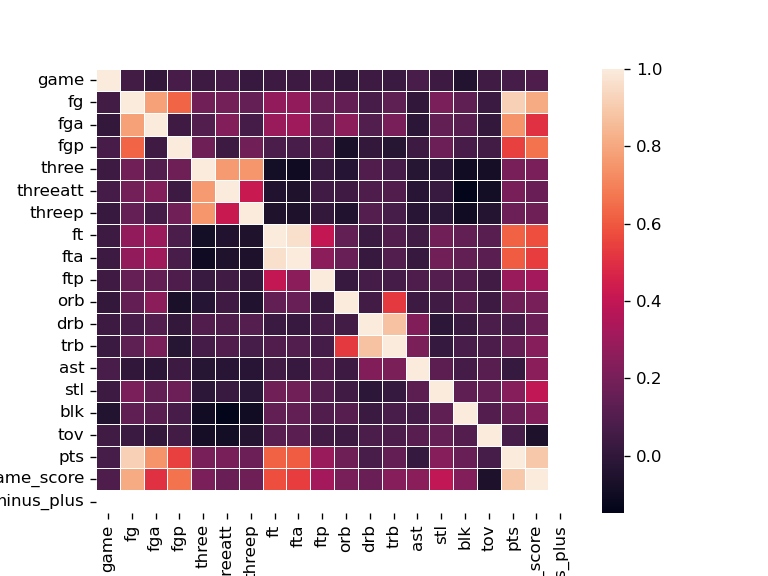
\includegraphics[width=0.65\linewidth]{correlation}
	\caption{Heatmap de correlacions}
	\label{fig:correlation}
\end{figure}\\
%Com influeix la normalització en la regressió?
\noindent
El fet de normalitzar les dades fa que els dominis dels atributs no desproporcionin la seva contribució al MSE, i això permet que funcioni millor el descens del gradient.\\
\\
%Com millora la regressió quan es filtren aquells atributs de les mostres que no contenen informació?
\noindent
%Si s'aplica un PCA, a quants components es redueix l'espai? Per què?
Hem fet un PCA i hem obtingut dues components principals. Per a fer-ho hem calculat la matriu de covariàncies pels atributs numèrics, i hem buscat els valors i vectors propis. Els valors propis ens diuen quanta informació hi ha en cada component: $w=(219.4, 29.6, 22.9, 15.3, 6.9, 4, 3.6, ...)$. Les dues primeres components tenen el 70,98\% i el 9,56\% d'informació respectivament.\\
\\
\noindent
%Amb quin atribut s'assoleix un MSE menor?
L'atribut que assoleix un MSE menor és el \textit{fg}. Aquest resultat no sorpren a ningú ja que estem predint els punts que farà a partir dels tirs anotats. El millor MSE i $R^2$ score l'obtenim fent servir les dades transformades pel PCA. A la següent taula recollim el MSE i el $R^2$ score de les dades normalitzades si fem una regressió agafant només un atribut, agafant-los tots i agafant els dos primers atributs del canvi del PCA:\\
\begin{table}[h!]
	\begin{center}
		\begin{tabular}{|c|c|c|}\hline
			Atribut	&	MSE	&	$R^2$ score	\\ \hline
			fg & 0.161090 & 0.849104 \\ \hline
			fga & 0.435080 & 0.592454 \\ \hline
			fgp & 0.787710 & 0.262141 \\ \hline
			%three & 1.058546 & 0.008445 \\ \hline
			%threeatt & 1.021708 & 0.042952 \\ \hline
			%threep & 1.072774 & -0.004883 \\ \hline
			ft & 0.627369 & 0.412334 \\ \hline
			fta & 0.639979 & 0.400523 \\ \hline
			ftp & 0.949395 & 0.110688 \\ \hline
			%orb & 1.037166 & 0.028472 \\ \hline
			%drb & 1.063142 & 0.004140 \\ \hline
			%trb & 1.045272 & 0.020879 \\ \hline
			%ast & 1.067689 & -0.000119 \\ \hline
			%stl & 0.983119 & 0.079099 \\ \hline
			%blk & 1.027546 & 0.037483 \\ \hline
			%tov & 1.059400 & 0.007645 \\ \hline
			game\_score & 0.219541 & 0.794353 \\ \hline
			Tots & 0.100316 & 0.895684 \\ \hline
			PCA $n=2$ & 0.092544 & 0.920129 \\ \hline
		\end{tabular}
	\end{center}
\end{table}\\
\newpage
\noindent
Finalment, veurem algunes regressions. Només hem pogut fer-les unidimensionals, les regressions amb tots els atributs i amb els que ha proporcionat el PCA no les hem pogut dibuixar.
\begin{figure}[!h]
	\centering
	\begin{subfigure}[b]{0.25\textwidth}
		\centering
		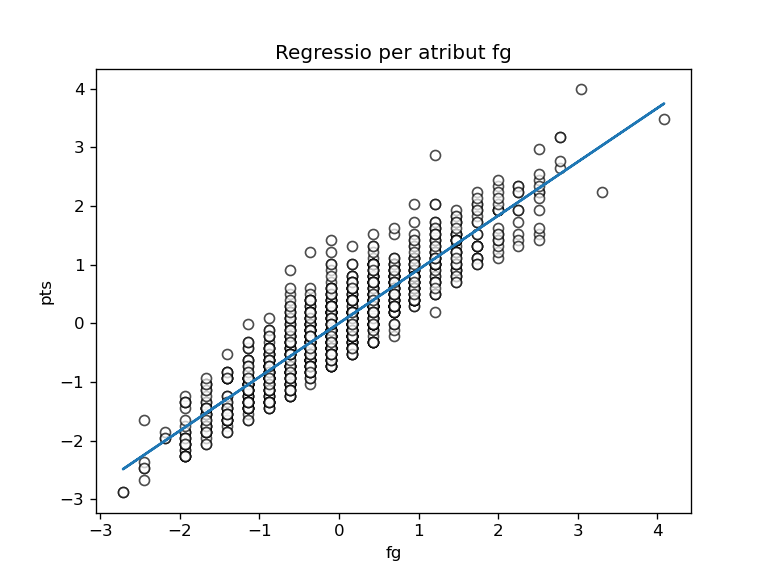
\includegraphics[width=\textwidth]{reg7}
		\caption*{Tirs anotats}
		\label{fig:reg7}
	\end{subfigure}
	\hfill
	\begin{subfigure}[b]{0.25\textwidth}
		\centering
		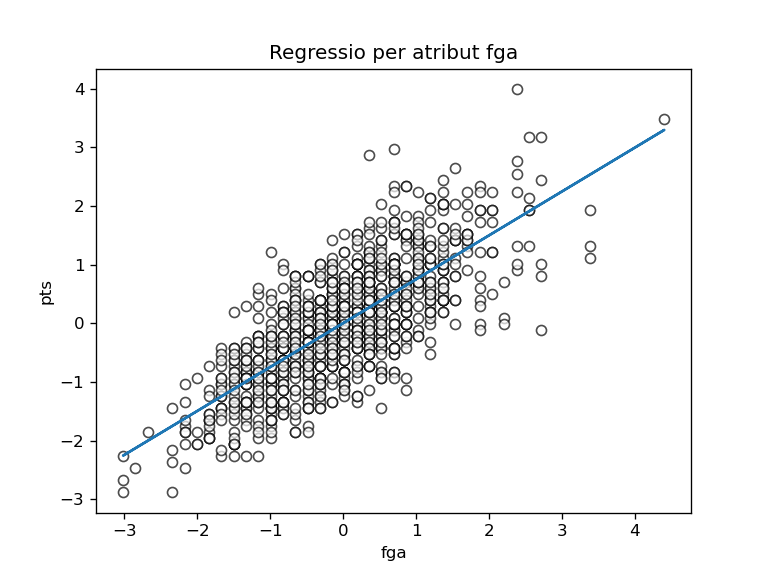
\includegraphics[width=\textwidth]{reg8}
		\caption*{Tirs intentats}
		\label{fig:hist23}
	\end{subfigure}
	\hfill
	\begin{subfigure}[b]{0.25\textwidth}
		\centering
		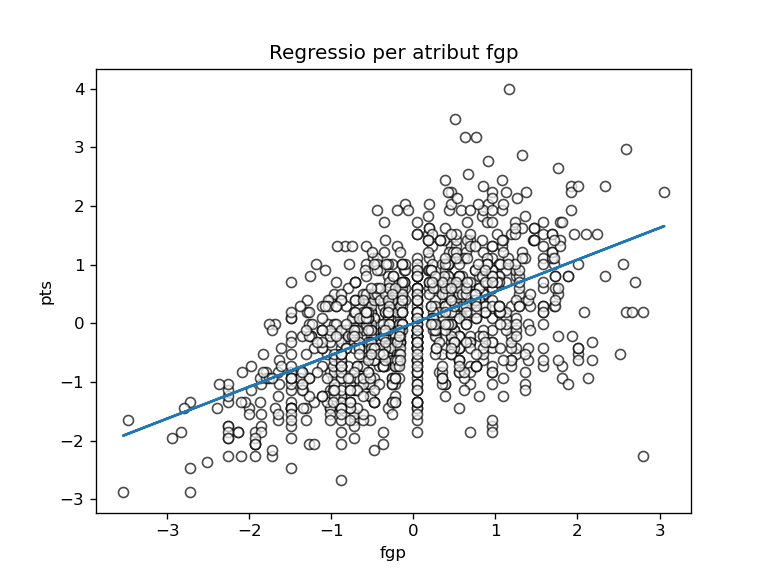
\includegraphics[width=\textwidth]{reg9}
		\caption*{Freqüència relativa tirs}
		\label{fig:hist24}
	\end{subfigure}
	\caption{Regressions amb un atribut}
	\label{fig:hist20}
\end{figure}
\begin{figure}[h!]
	\centering
	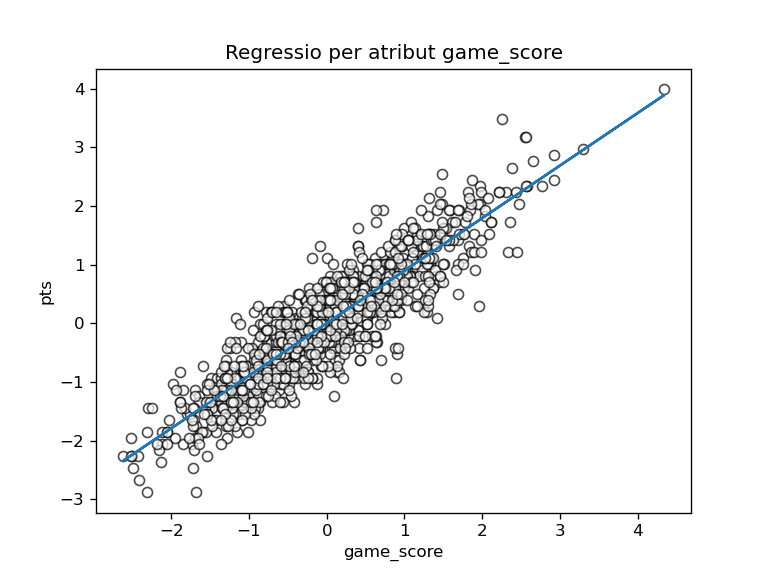
\includegraphics[width=0.5\linewidth]{reg24}
	\caption{Regressió amb game\_score}
	\label{fig:correlation}
\end{figure}\\

\end{document}
